\documentclass[9pt,letterpaper]{article}
%\usepackage[utf8]{inputenc}
\UseRawInputEncoding
\usepackage[english]{babel}
\usepackage{listings}
\usepackage{xcolor}
\usepackage{graphicx}

%For syntax highlighting
\definecolor{codegreen}{rgb}{0,0.6,0}
\definecolor{codegray}{rgb}{0.5,0.5,0.5}
\definecolor{codepurple}{rgb}{0.58,0,0.82}
\definecolor{backcolour}{rgb}{1,1,1}

%%Sets different parameters
\lstdefinestyle{mystyle}{
    backgroundcolor=\color{backcolour},   
    commentstyle=\color{codegreen},
    keywordstyle=\color{magenta},
    numberstyle=\tiny\color{codegray},
    stringstyle=\color{codepurple},
    basicstyle=\ttfamily\footnotesize,
    breakatwhitespace=false,         
    breaklines=true,                 
    captionpos=b,                    
    keepspaces=true,                 
    numbers=left,                    
    numbersep=5pt,                  
    showspaces=false,                
    showstringspaces=false,
    showtabs=false,                  
    tabsize=4
}
\lstset{style=mystyle}

\title{\textbf{Department of Computer Science and Engineering}}
\author{\textbf{Shivanirudh S G, 185001146, Semester VII }}

\date{12 August 2021}

\begin{document}
\maketitle
\hrule
\section*{\center{UCS1712 - Graphics and Multimedia Lab}}
\hrule 
\bigskip\bigskip

%Assignment name
\subsection*{\center{\textbf{Exercise 5: 2D Transformations in C++ using OpenGL}}}

%Objective
\subsection*{\flushleft{Aim:}}
\begin{flushleft}
     To apply the 2D transformations on objects and to render the final output along with the original object.  
\end{flushleft}

%Code
\subsection*{\flushleft{Code:}}
\begin{flushleft}
\lstinputlisting[language = C++]{Headers.h}
\lstinputlisting[language = C++]{Signatures.h}
\lstinputlisting[language = C++]{Helpers.h}
\lstinputlisting[language = C++]{main.cpp}
\end{flushleft}
\newpage
\subsection*{\flushleft{Output:}}
\textbf{Original Image:}\\
Choose number of edges: (1 for line, 3 and upwards for polygon): 5\\
Enter vertices:\\ 
Vertex 1 (x,y): 30 30\\
Vertex 2 (x,y): 10 60\\
Vertex 3 (x,y): 60 80\\
Vertex 4 (x,y): 110 60\\
Vertex 5 (x,y): 90 30\\
Number of edges: 5\\
\begin{figure}[h]
    \centering
    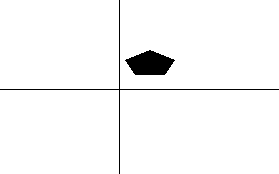
\includegraphics[height=5cm]{Outputs/OP1.png}
\end{figure}

\newpage
\textbf{\large{Translation:}}

Choose transformation: \\
1 for Translation\\
2 for Rotation\\
3 for Scaling\\
4 for Reflection\\
5 for shearing\\
0 to Exit\\
Enter your choice: 1\\
\\
Enter the translation factor for X and Y: 30 30\\
\begin{figure}[h]
    \centering
    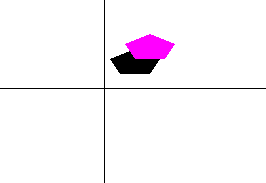
\includegraphics[height=5cm]{Outputs/OP2.png}
\end{figure}

\newpage
\textbf{\large{Rotation: }}\\
\textbf{About origin:}\\

Enter the rotation angle: 45\\
Enter point about which to be rotated: 0 0\\

\begin{figure}[h]
    \centering
    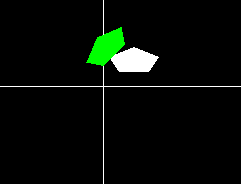
\includegraphics[height=5cm]{Outputs/OP3.png}
\end{figure}

\textbf{About fixed point:}\\

Enter the rotation angle: 45\\
Enter point about which to be rotated: 60 80\\

\begin{figure}[h]
    \centering
    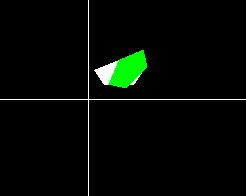
\includegraphics[height=5cm]{Outputs/OP4.png}
\end{figure}


\newpage
\textbf{\large{Scaling: }}\\
\textbf{About origin - Uniform:}\\

Enter the scaling factor for X and Y: 3 3\\
Enter point about which to be scaled: 0 0

\begin{figure}[h]
    \centering
    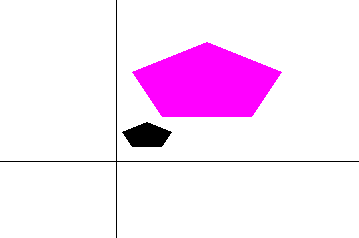
\includegraphics[height=5cm]{Outputs/OP5.png}
\end{figure}

\textbf{About origin - Differential:}

Enter the scaling factor for X and Y: 2 4\\
Enter point about which to be scaled: 0 0

\begin{figure}[h]
    \centering
    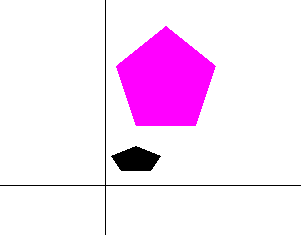
\includegraphics[height=5cm]{Outputs/OP6.png}
\end{figure}

\newpage
\textbf{About fixed point:}

Enter the scaling factor for X and Y: 3 3\\
Enter point about which to be scaled: 100 100

\begin{figure}[h]
    \centering
    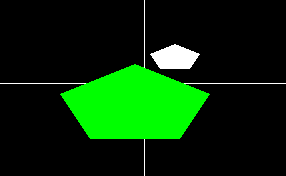
\includegraphics[height=5cm]{Outputs/OP7.png}
\end{figure}

\newpage
\textbf{\large{Reflection: }}\\
\textbf{With respect to X-axis:}

Enter the angle with X-axis and Y-intercept of the mirror: 0 0

\begin{figure}[h]
    \centering
    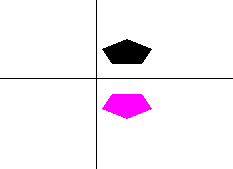
\includegraphics[height=5cm]{Outputs/OP8.png}
\end{figure}

\textbf{With respect to Y-axis:}

Enter the angle with X-axis and Y-intercept of the mirror: 90 0

\begin{figure}[h]
    \centering
    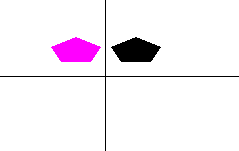
\includegraphics[height=5cm]{Outputs/OP9.png}
\end{figure}

\newpage
\textbf{With respect to origin:}

Enter the angle with X-axis and Y-intercept of the mirror: 135 0

\begin{figure}[h]
    \centering
    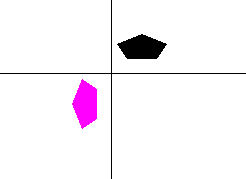
\includegraphics[height=5cm]{Outputs/OP10.png}
\end{figure}

\textbf{With respect to line x=y:}

Enter the angle with X-axis and Y-intercept of the mirror: 45 0

\begin{figure}[h]
    \centering
    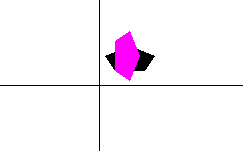
\includegraphics[height=5cm]{Outputs/OP11.png}
\end{figure}

\newpage
\textbf{\large{Shearing: }}\\
\textbf{X-direction:}\\

Enter the shearing factor for X and Y: 3 0

\begin{figure}[h]
    \centering
    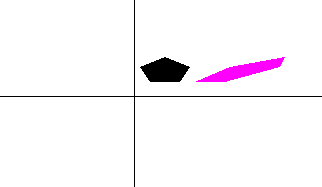
\includegraphics[height=5cm]{Outputs/OP12.png}
\end{figure}

\textbf{Y-direction:}\\

Enter the shearing factor for X and Y: 0 3

\begin{figure}[h]
    \centering
    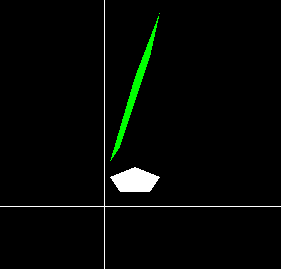
\includegraphics[height=5cm]{Outputs/OP13.png}
\end{figure}

\newpage
\textbf{Both X and Y directions:}\\

Enter the shearing factor for X and Y: 3 3

\begin{figure}[h]
    \centering
    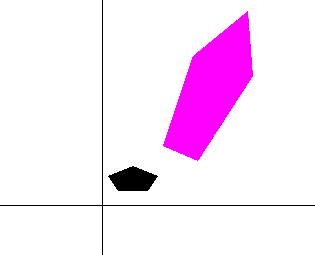
\includegraphics[height=5cm]{Outputs/OP14.png}
\end{figure}

\bigskip\bigskip
\hrule

\end{document}